%=============================================================================
%  RTS Backward Smoother -- Mathematical Notes & Documentation
%  smoother.py | Project Dark-Wing
%  Financial Mathematics / Time Series Analysis / Kalman_Filter
%=============================================================================
\documentclass[10pt,a4paper,twocolumn]{article}

%--- Geometry ----------------------------------------------------------------
\usepackage[a4paper,top=1.8cm,bottom=1.8cm,left=1.5cm,right=1.5cm,
            columnsep=0.7cm]{geometry}

%--- Math --------------------------------------------------------------------
\usepackage{amsmath,amssymb,amsthm,mathtools}

%--- Typography --------------------------------------------------------------
\usepackage[T1]{fontenc}
\usepackage{lmodern}
\usepackage{microtype}
\usepackage{parskip}
\setlength{\parskip}{2pt}

%--- Colours -----------------------------------------------------------------
\usepackage{xcolor}
\definecolor{codebg}{RGB}{245,247,250}
\definecolor{codeframe}{RGB}{180,195,220}
\definecolor{keyword}{RGB}{0,80,180}
\definecolor{comment}{RGB}{80,115,80}
\definecolor{string}{RGB}{160,40,20}
\definecolor{mathbluebg}{RGB}{230,240,255}
\definecolor{mathblue}{RGB}{10,60,160}
\definecolor{accent}{RGB}{25,95,195}
\definecolor{greenbg}{RGB}{230,250,232}
\definecolor{greenframe}{RGB}{50,155,70}
\definecolor{yellowbg}{RGB}{255,252,230}
\definecolor{yellowframe}{RGB}{180,150,0}
\definecolor{notebg}{RGB}{248,245,255}
\definecolor{noteframe}{RGB}{120,80,180}

%--- Code listings -----------------------------------------------------------
\usepackage{listings}
\lstdefinestyle{python}{
  language=Python,
  backgroundcolor=\color{codebg},
  frame=single,rulecolor=\color{codeframe},
  basicstyle=\ttfamily\fontsize{6.5}{8}\selectfont,
  keywordstyle=\bfseries\color{keyword},
  commentstyle=\itshape\color{comment},
  stringstyle=\color{string},
  numbers=left,numberstyle=\tiny\color{gray!70},
  numbersep=4pt,breaklines=true,tabsize=2,
  showstringspaces=false,aboveskip=3pt,belowskip=3pt,
  xleftmargin=12pt,
}
\lstdefinestyle{pythonplain}{
  language=Python,
  backgroundcolor=\color{codebg},
  frame=single,rulecolor=\color{codeframe},
  basicstyle=\ttfamily\fontsize{6.5}{8}\selectfont,
  keywordstyle=\bfseries\color{keyword},
  commentstyle=\itshape\color{comment},
  stringstyle=\color{string},
  numbers=none,breaklines=true,tabsize=2,
  showstringspaces=false,aboveskip=3pt,belowskip=3pt,
  xleftmargin=4pt,
}

%--- TikZ --------------------------------------------------------------------
\usepackage{tikz}
\usetikzlibrary{shapes.geometric,arrows.meta,positioning,calc,
                backgrounds,decorations.pathreplacing,fit}
\raggedbottom

\tikzset{
  fc_start/.style={rectangle,rounded corners=5pt,
    draw=accent,fill=accent!18,
    text width=4.4cm,align=center,
    font=\footnotesize\bfseries,
    inner sep=4pt,minimum height=0.6cm},
  fc_proc/.style={rectangle,
    draw=black!55,fill=white,
    text width=4.4cm,align=center,
    font=\footnotesize,
    inner sep=3pt,minimum height=0.58cm},
  fc_dec/.style={diamond,aspect=2.5,
    draw=accent,fill=accent!9,
    text width=2.9cm,align=center,
    font=\fontsize{6.2}{7.2}\selectfont,
    inner sep=1pt},
  fc_out/.style={rectangle,rounded corners=3pt,
    draw=greenframe,fill=greenbg,
    text width=4.4cm,align=center,
    font=\footnotesize,
    inner sep=3pt,minimum height=0.58cm},
  fc_side/.style={rectangle,
    draw=black!45,fill=yellow!10,
    text width=2.0cm,align=center,
    font=\fontsize{6.2}{7.2}\selectfont,
    inner sep=2pt,minimum height=0.52cm},
  arr/.style={-Stealth,semithick,draw=black!65},
}

%--- Boxes -------------------------------------------------------------------
\usepackage[most]{tcolorbox}
\tcbset{
  mathbox/.style={colback=mathbluebg,colframe=mathblue,
    fonttitle=\bfseries\small,title=#1,
    boxrule=0.5pt,top=3pt,bottom=3pt,left=4pt,right=4pt,
    before skip=4pt,after skip=4pt},
  exbox/.style={colback=yellowbg,colframe=yellowframe,
    fonttitle=\bfseries\small,title=#1,
    boxrule=0.5pt,top=3pt,bottom=3pt,left=4pt,right=4pt,
    before skip=4pt,after skip=4pt},
  resultbox/.style={colback=greenbg,colframe=greenframe,
    fonttitle=\bfseries\small,title=#1,
    boxrule=0.5pt,top=3pt,bottom=3pt,left=4pt,right=4pt,
    before skip=4pt,after skip=4pt},
  codebox/.style={colback=codebg,colframe=codeframe,
    fonttitle=\bfseries\small\color{accent},title=#1,
    boxrule=0.5pt,top=2pt,bottom=2pt,left=2pt,right=2pt,
    before skip=4pt,after skip=4pt},
  notebox/.style={colback=notebg,colframe=noteframe,
    fonttitle=\bfseries\small,title=#1,
    boxrule=0.5pt,top=3pt,bottom=3pt,left=4pt,right=4pt,
    before skip=4pt,after skip=4pt},
}

%--- Tables ------------------------------------------------------------------
\usepackage{booktabs,array,multirow}

%--- Header / Footer ---------------------------------------------------------
\usepackage{fancyhdr}
\usepackage[hidelinks]{hyperref}
\pagestyle{fancy}\fancyhf{}
\fancyhead[L]{\footnotesize\textbf{RTS Backward Smoother --- smoother.py}}
\fancyhead[R]{\footnotesize Project Dark-Wing}
\fancyfoot[C]{\footnotesize\thepage}
\renewcommand{\headrulewidth}{0.4pt}

%--- Floats / Captions -------------------------------------------------------
\usepackage{float,caption,graphicx}
\captionsetup{font=scriptsize,labelfont=bf,skip=3pt}

%--- Section formatting ------------------------------------------------------
\usepackage{titlesec}
\titlespacing*{\section}{0pt}{7pt}{3pt}
\titlespacing*{\subsection}{0pt}{5pt}{2pt}
\titlespacing*{\subsubsection}{0pt}{3pt}{1pt}
\titleformat{\section}{\normalfont\bfseries\color{accent}}{}{0em}{}
  [{\color{accent}\titlerule[0.5pt]}]
\titleformat{\subsection}{\normalfont\bfseries\small}{}{0em}{}
\titleformat{\subsubsection}{\normalfont\itshape\small}{}{0em}{}

%=============================================================================
\begin{document}
%=============================================================================

\twocolumn[{%
\begin{center}
  {\LARGE\bfseries\color{accent}
    RTS Backward Smoother --- Mathematical Notes \& Documentation}\\[5pt]
  {\large\bfseries Rauch--Tung--Striebel Smoother for Dynamic Hedge Ratio Estimation}\\[3pt]
  {\small\itshape Module: \texttt{smoother.py} \quad|\quad
   Full Derivation, Numerical Example, and Python Implementation}\\[3pt]
  {\small Project Dark-Wing \quad|\quad \today}
\end{center}
\vspace{4pt}
\noindent\rule{\linewidth}{0.5pt}\vspace{2pt}
\begin{quote}\small
\textbf{Abstract.}~The Kalman filter is a \emph{causal} estimator: at each
time $t$ it computes $\hat{\beta}_{t|t} = \mathbb{E}[\beta_t \mid Y_1,\ldots,Y_t]$
using only past and present observations.  The
\textbf{Rauch--Tung--Striebel (RTS) smoother} is a non-causal
\emph{backward} pass that refines every estimate by incorporating all
$T$ available observations, yielding $\hat{\beta}_{t|T} =
\mathbb{E}[\beta_t \mid Y_1,\ldots,Y_T]$.  Because the smoother has
access to future data it is strictly more informative than the filter,
producing lower-variance, smoother hedge-ratio trajectories.  This
document derives the RTS recursion from first principles, proves the
variance reduction bound $R_t = 1 - P_{t|T}/P_{t|t} \in [0,1]$,
provides a four-step numerical walkthrough, and documents every method
of the \texttt{KalmanSmoother} Python class.  The smoother's role in
EM-based parameter estimation and its position at Step~6.1 in the
Dark-Wing pipeline are also covered.
\end{quote}
\noindent\rule{\linewidth}{0.5pt}\vspace{5pt}
}]

%=============================================================================
\section{Why Smooth? --- Filter vs.\ Smoother}
%=============================================================================

\subsection{The Information Gap}

The Kalman \emph{filter} answers the question:
\begin{quote}\itshape
  ``Given everything seen so far, what is the best estimate of $\beta_t$?''
\end{quote}
This causal (online) estimate is essential for real-time trading.
In backtesting and research, however, the full series
$Y_1,\ldots,Y_T$ is already in memory.  Discarding future information
is wasteful.  The \emph{smoother} answers:
\begin{quote}\itshape
  ``Given the entire dataset, what is the best possible estimate of $\beta_t$?''
\end{quote}

\begin{tcolorbox}[notebox={Filter vs.\ Smoother: Information Set}]
\begin{align*}
  \hat{\beta}_{t|t}
    &= \mathbb{E}[\beta_t \mid Y_1,\ldots,Y_t]
    \quad\text{(filter, causal)}\\
  \hat{\beta}_{t|T}
    &= \mathbb{E}[\beta_t \mid Y_1,\ldots,Y_T]
    \quad\text{(smoother, non-causal)}
\end{align*}
Since $\{Y_1,\ldots,Y_t\} \subseteq \{Y_1,\ldots,Y_T\}$, the smoother
uses a strictly larger information set for all $t < T$.
\end{tcolorbox}

\subsection{Variance Reduction}

The smoother's posterior variance is \emph{never larger} than the filter's.

\begin{tcolorbox}[mathbox={Variance Ordering (Law of Total Variance)}]
\vspace{-4pt}
\begin{equation}\label{eq:var_order}
  P_{t|T} \;\leq\; P_{t|t} \quad \forall\; t
\end{equation}
\vspace{-4pt}
Proof sketch:
\[
  \underbrace{\mathrm{Var}(\beta_t \mid Y_{1:t})}_{P_{t|t}}
  = \mathbb{E}[P_{t|T} \mid Y_{1:t}]
  + \mathrm{Var}(\hat\beta_{t|T} \mid Y_{1:t})
  \;\geq\; P_{t|T}
\]
\end{tcolorbox}

The \textbf{variance reduction ratio}:

\begin{tcolorbox}[mathbox={Variance Reduction Ratio}]
\vspace{-3pt}
\begin{equation}\label{eq:vr}
  R_t = 1 - \frac{P_{t|T}}{P_{t|t}} \;\in\; [0, 1]
\end{equation}
\vspace{-4pt}
$R_t = 0$: smoother adds nothing. $R_t = 1$: state perfectly known.
$R_t$ is largest early in the series (cold filter) and is identically
$0$ at $t = T$ by construction.
\end{tcolorbox}

%=============================================================================
\section{State-Space Model}
%=============================================================================

\subsection{Univariate Dynamic Hedge-Ratio Model}

\begin{tcolorbox}[mathbox={State-Space Model (scalar)}]
\vspace{-4pt}
\begin{align}
  \text{Obs.:}\quad
    Y_t &= \beta_t\,X_t + \varepsilon_t,
    \quad \varepsilon_t \sim \mathcal{N}(0, R) \label{eq:obs}\\
  \text{State:}\quad
    \beta_t &= \beta_{t-1} + \eta_t,
    \quad \eta_t \sim \mathcal{N}(0, Q) \label{eq:state}
\end{align}
\vspace{-4pt}
$(Y_t, X_t)$ is the cointegrated pair; $\beta_t$ is the time-varying
hedge ratio.  Transition matrix $\mathbf{T}=1$ (random walk on $\beta$).
$Q$: process noise; $R$: obs.\ noise.
\end{tcolorbox}

The Kalman filter forward pass stores at every $t$:
\begin{itemize}\setlength\itemsep{0pt}
  \item $\hat{\beta}_{t|t}$, $P_{t|t}$ --- filtered state and variance
  \item $\hat{\beta}_{t+1|t}$, $P_{t+1|t}$ --- one-step predictions
\end{itemize}

\subsection{Kalman Filter Prediction Recap}

\begin{tcolorbox}[mathbox={KF Prediction (forward pass)}]
\vspace{-4pt}
\begin{align}
  \hat{\beta}_{t+1|t} &= \hat{\beta}_{t|t}
    \quad\text{(since $\mathbf{T}=1$)} \\
  P_{t+1|t} &= P_{t|t} + Q
\end{align}
\vspace{-4pt}
Predicted variance grows by $Q$ each step.  The stored
$P_{t+1|t}$ values are consumed by the backward smoother pass.
\end{tcolorbox}

%=============================================================================
\section{RTS Algorithm Derivation}
%=============================================================================

\subsection{Joint Gaussian at Time $t$}

Conditionally on $Y_{1:t}$, the joint distribution of
$(\beta_t, \beta_{t+1})$ is Gaussian:
\[
  \begin{pmatrix}\beta_t\\\beta_{t+1}\end{pmatrix}
  \Biggm| Y_{1:t}
  \;\sim\;
  \mathcal{N}\!\left(
    \begin{pmatrix}\hat\beta_{t|t}\\\hat\beta_{t+1|t}\end{pmatrix},\;
    \begin{pmatrix}P_{t|t} & P_{t|t}\\P_{t|t} & P_{t+1|t}\end{pmatrix}
  \right)
\]
The cross-covariance equals $P_{t|t}$ because
$\mathrm{Cov}(\beta_t,\,\beta_t+\eta_t) = P_{t|t}$ (since
$\eta_t \perp Y_{1:t}$, $\mathbf{T}=1$).

\subsection{Formula 1 --- Smoothing Gain $\Xi_t$}

Applying the standard bivariate-Gaussian conditional-mean
formula and incorporating the updated $\hat\beta_{t+1|T}$:

\begin{tcolorbox}[mathbox={Formula 1 --- Smoothing Gain (scalar)}]
\vspace{-4pt}
\begin{equation}\label{eq:xi}
  \boxed{\Xi_t \;=\; \frac{P_{t|t}}{P_{t+1|t}}}
\end{equation}
\vspace{-4pt}
\textbf{General (multivariate)} case:
$\boldsymbol{\Xi}_t = P_{t|t}\,\mathbf{T}^\top P_{t+1|t}^{-1}$.
With $\mathbf{T}=1$ this reduces to Eq.~\eqref{eq:xi}.\\[2pt]
Since $P_{t+1|t} = P_{t|t}+Q \geq P_{t|t} > 0$, we have
$\Xi_t \in (0,1]$ always.  A larger $Q$ reduces $\Xi_t$,
dampening the backward correction.
\end{tcolorbox}

\subsection{Formula 2 --- Smoothed State}

\begin{tcolorbox}[mathbox={Formula 2 --- Smoothed State}]
\vspace{-4pt}
\begin{equation}\label{eq:smooth_state}
  \boxed{
    \hat\beta_{t|T} \;=\; \hat\beta_{t|t}
      + \Xi_t\,\bigl(\hat\beta_{t+1|T} - \hat\beta_{t+1|t}\bigr)
  }
\end{equation}
\vspace{-3pt}
The term $(\hat\beta_{t+1|T} - \hat\beta_{t+1|t})$ is the
``smoothed innovation'' at $t+1$: how much future data
shifted the estimate of $\beta_{t+1}$.  This is propagated
back to time $t$, attenuated by $\Xi_t \leq 1$.
\begin{itemize}\setlength\itemsep{0pt}
  \item Innovation $> 0$: future data saw $\beta$ higher; increase $\hat\beta_{t|T}$.
  \item Innovation $= 0$: no backward correction.
  \item $\Xi_t \to 0$ (large $Q$): corrections do not propagate.
\end{itemize}
\end{tcolorbox}

\subsection{Formula 3 --- Smoothed Covariance}

\begin{tcolorbox}[mathbox={Formula 3 --- Smoothed Covariance}]
\vspace{-4pt}
\begin{equation}\label{eq:smooth_cov}
  \boxed{
    P_{t|T} \;=\; P_{t|t}
      - \Xi_t\,\bigl(P_{t+1|t} - P_{t+1|T}\bigr)\,\Xi_t
  }
\end{equation}
\vspace{-3pt}
\textbf{Derivation sketch}: From the conditional variance of
the bivariate Gaussian, expanding the formula for the
conditional covariance given $\beta_{t+1|T}$:
\[
  P_{t|T}
  = P_{t|t} - \Xi_t P_{t+1|t}\Xi_t + \Xi_t P_{t+1|T}\Xi_t
\]
Since $P_{t+1|T} \leq P_{t+1|t}$ (induction), the correction
$\Xi_t(P_{t+1|t}-P_{t+1|T})\Xi_t \geq 0$, so $P_{t|T} \leq P_{t|t}$.
\end{tcolorbox}

\subsection{Full RTS Recursion}

\begin{tcolorbox}[resultbox={Complete RTS Algorithm}]
\textbf{Initialise} ($t = T-1$):
$\hat\beta_{T-1|T} = \hat\beta_{T-1|T-1}$,\;
$P_{T-1|T} = P_{T-1|T-1}$.\\[4pt]
\textbf{Backward loop} for $t = T-2,\,T-3,\,\ldots,\,0$:
\begin{enumerate}\setlength\itemsep{2pt}
  \item $\Xi_t = P_{t|t} / P_{t+1|t}$
        \hfill\textit{(smoothing gain)}
  \item $\hat\beta_{t|T} = \hat\beta_{t|t}
          + \Xi_t\,(\hat\beta_{t+1|T} - \hat\beta_{t+1|t})$
        \hfill\textit{(smoothed state)}
  \item $P_{t|T} = P_{t|t}
          - \Xi_t\,(P_{t+1|t} - P_{t+1|T})\,\Xi_t$
        \hfill\textit{(smoothed variance)}
\end{enumerate}
\textbf{Complexity}: $\mathcal{O}(T)$ --- one backward sweep.
\end{tcolorbox}

%=============================================================================
\section{Variance Reduction Analysis}
%=============================================================================

\subsection{Formal Proof that $R_t \in [0,1]$}

\begin{tcolorbox}[mathbox={Proof: {$R_t \in [0,1]$}}]
\textbf{Lower bound ($R_t \geq 0$, i.e.\ $P_{t|T} \leq P_{t|t}$)}:

\noindent From Eq.~\eqref{eq:smooth_cov}:
\[
  P_{t|T} = P_{t|t} - \underbrace{\Xi_t^2\,(P_{t+1|t}-P_{t+1|T})}_{\geq\,0}
  \;\leq\; P_{t|t}
\]
The term is $\geq 0$ because $P_{t+1|t} \geq P_{t+1|T}$ by induction
(base case: $P_{T|T} = P_{T|T}$) and $\Xi_t^2 \geq 0$.

\textbf{Upper bound ($R_t \leq 1$, i.e.\ $P_{t|T} \geq 0$)}:

\noindent Rewrite Eq.~\eqref{eq:smooth_cov}:
\[
  P_{t|T} = P_{t|t}(1 - \Xi_t^2) + \Xi_t^2\,P_{t+1|T} \geq 0
\]
since $\Xi_t \leq 1 \Rightarrow 1-\Xi_t^2 \geq 0$, and
$P_{t+1|T} \geq 0$ by induction. $\blacksquare$
\end{tcolorbox}

\subsection{Process Noise Regime Analysis}

\begin{center}\small
\begin{tabular}{@{}lll@{}}
\toprule
Regime & $Q$ & Smoother behaviour\\\midrule
Near-constant $\beta$ & $Q \to 0$ & $\Xi_t \to 1$; large backward corrections\\
Freely evolving $\beta$ & $Q \to \infty$ & $\Xi_t \to 0$; no correction\\
Tuned $Q$ & Optimal & $R_t \in [0.2,0.6]$; balanced estimates\\
\bottomrule
\end{tabular}
\end{center}

%=============================================================================
\section{Financial Interpretation}
%=============================================================================

\subsection{When to Use Filter vs.\ Smoother}

\begin{center}\small
\begin{tabular}{@{}p{1.7cm}p{2.3cm}p{2.3cm}@{}}
\toprule
\textbf{Criterion} & \textbf{Kalman Filter} & \textbf{RTS Smoother}\\\midrule
Causality       & Causal (online)        & Non-causal (offline)\\
Data used       & $Y_1,\ldots,Y_t$       & $Y_1,\ldots,Y_T$\\
Real-time?      & \textcolor{greenframe}{\textbf{Yes}}
                & \textcolor{red}{\textbf{No}}\\
Variance        & $P_{t|t}$              & $P_{t|T} \leq P_{t|t}$\\\midrule
Use case 1      & Live trade signals     & Backtest research\\
Use case 2      & Position sizing        & Signal calibration\\
Use case 3      & Risk monitoring        & EM parameter tuning\\
Use case 4      & Streaming data         & Offline spread study\\\midrule
Dark-Wing file  & \texttt{kalman\_filter.py}
                & \texttt{smoother.py}\\
\bottomrule
\end{tabular}
\end{center}

\subsection{Smoothed Spread for Backtesting}

\begin{tcolorbox}[mathbox={Smoothed Spread}]
\vspace{-4pt}
\begin{equation}
  S_t^{\text{smooth}} = Y_t - \hat\beta_{t|T}\,X_t
\end{equation}
\vspace{-3pt}
Contrast with the filtered spread
$S_t^{\text{filt}} = Y_t - \hat\beta_{t|t}\,X_t$.
The smoothed spread is less noisy and has more stable
mean-reversion properties, making it preferable for
calibrating entry/exit z-score thresholds in backtests.
\end{tcolorbox}

\subsection{Look-Ahead Bias Warning}

\begin{tcolorbox}[notebox={Do NOT Trade on Smoothed $\hat\beta_{t|T}$}]
The smoother requires $\hat\beta_{t+1|T}$, available only
\emph{after} observing all $T$ data points.  Using smoothed
quantities as live trading signals constitutes
\textbf{look-ahead bias}: unrealistically good backtest PnL
that vanishes in production.  \texttt{KalmanSmoother} is a
\textbf{research and parameter calibration tool only}.
\end{tcolorbox}

%=============================================================================
\section{Worked Numerical Example (4 Timesteps)}
%=============================================================================

\begin{tcolorbox}[exbox={Setup}]
$Q = 0.01$,\; $R = 0.1$,\; $\beta_0 = 1.0$,\; $P_0 = 1.0$.\\[3pt]
Observation pairs $(Y_t, X_t)$:
$(2.1,\,2.0)$,\; $(3.3,\,3.0)$,\; $(2.5,\,2.4)$,\; $(4.2,\,4.0)$.\\[3pt]
The Kalman filter forward pass has been run, producing the
stored quantities below ($T=4$, indices $t=0,1,2,3$).
\end{tcolorbox}

\subsubsection{Forward Pass Storage}

\begin{center}\small
\begin{tabular}{@{}ccccc@{}}
\toprule
$t$ & $\hat\beta_{t|t}$ & $P_{t|t}$
    & $\hat\beta_{t+1|t}$ & $P_{t+1|t}$\\\midrule
0 & 1.050 & 0.048 & 1.050 & 0.058\\
1 & 1.097 & 0.031 & 1.097 & 0.041\\
2 & 1.036 & 0.025 & 1.036 & 0.035\\
3 & 1.048 & 0.021 & ---   & ---\\
\bottomrule
\end{tabular}
\end{center}
\noindent($P_{t+1|t} = P_{t|t} + Q$,\; $Q = 0.01$.)

\subsubsection{Step $t=3$: Initialise Smoother}

\begin{tcolorbox}[exbox={Boundary Condition}]
At $t = T-1 = 3$, smoothed equals filtered:
\[
  \hat\beta_{3|T} = \hat\beta_{3|3} = 1.048,
  \quad P_{3|T} = P_{3|3} = 0.021
\]
\end{tcolorbox}

\subsubsection{Step $t=2$}

\begin{tcolorbox}[exbox={Backward Step at {$t=2$}}]
\textbf{Gain:} $\Xi_2 = 0.025 / 0.035 = 0.714$\\[3pt]
\textbf{State:}
\[
  \hat\beta_{2|T} = 1.036 + 0.714\,(1.048 - 1.036)
                  = 1.036 + 0.009 = 1.045
\]
\textbf{Covariance:}
\[
  P_{2|T} = 0.025 - 0.714\,(0.035 - 0.021)\,0.714 = 0.018
\]
\end{tcolorbox}

\subsubsection{Step $t=1$}

\begin{tcolorbox}[exbox={Backward Step at {$t=1$}}]
\textbf{Gain:} $\Xi_1 = 0.031 / 0.041 = 0.756$\\[3pt]
\textbf{State:}
\begin{align*}
  \hat\beta_{1|T} &= 1.097 + 0.756\,(1.045 - 1.036)\\
                  &= 1.097 + 0.007 = 1.104
\end{align*}
\textbf{Covariance:}
\[
  P_{1|T} = 0.031 - 0.756\,(0.041 - 0.018)\,0.756 = 0.018
\]
\end{tcolorbox}

\subsubsection{Step $t=0$}

\begin{tcolorbox}[exbox={Backward Step at {$t=0$}}]
\textbf{Gain:} $\Xi_0 = 0.048 / 0.058 = 0.828$\\[3pt]
\textbf{State:}
\begin{align*}
  \hat\beta_{0|T} &= 1.050 + 0.828\,(1.104 - 1.097)\\
                  &= 1.050 + 0.006 = 1.056
\end{align*}
\textbf{Covariance:}
\[
  P_{0|T} = 0.048 - 0.828\,(0.058 - 0.018)\,0.828 = 0.021
\]
\end{tcolorbox}

\subsubsection{Summary}

\begin{tcolorbox}[resultbox={Numerical Example Summary}]
\begin{center}\small
\begin{tabular}{@{}cccccc@{}}
\toprule
$t$ & $\hat\beta_{t|t}$ & $\hat\beta_{t|T}$
    & $P_{t|t}$ & $P_{t|T}$ & $R_t$\\\midrule
0 & 1.050 & 1.056 & 0.048 & 0.021 & 0.563\\
1 & 1.097 & 1.104 & 0.031 & 0.018 & 0.419\\
2 & 1.036 & 1.045 & 0.025 & 0.018 & 0.280\\
3 & 1.048 & 1.048 & 0.021 & 0.021 & 0.000\\
\bottomrule
\end{tabular}
\end{center}
$R_t > 0$ for $t < T$; $R_3 = 0$ by construction.
Variance reduction is largest at $t=0$ (cold filter).
\end{tcolorbox}

%=============================================================================
\section{TikZ Flowchart --- \texttt{KalmanSmoother}}
%=============================================================================

\begin{figure}[H]
\centering
\resizebox{\columnwidth}{!}{%
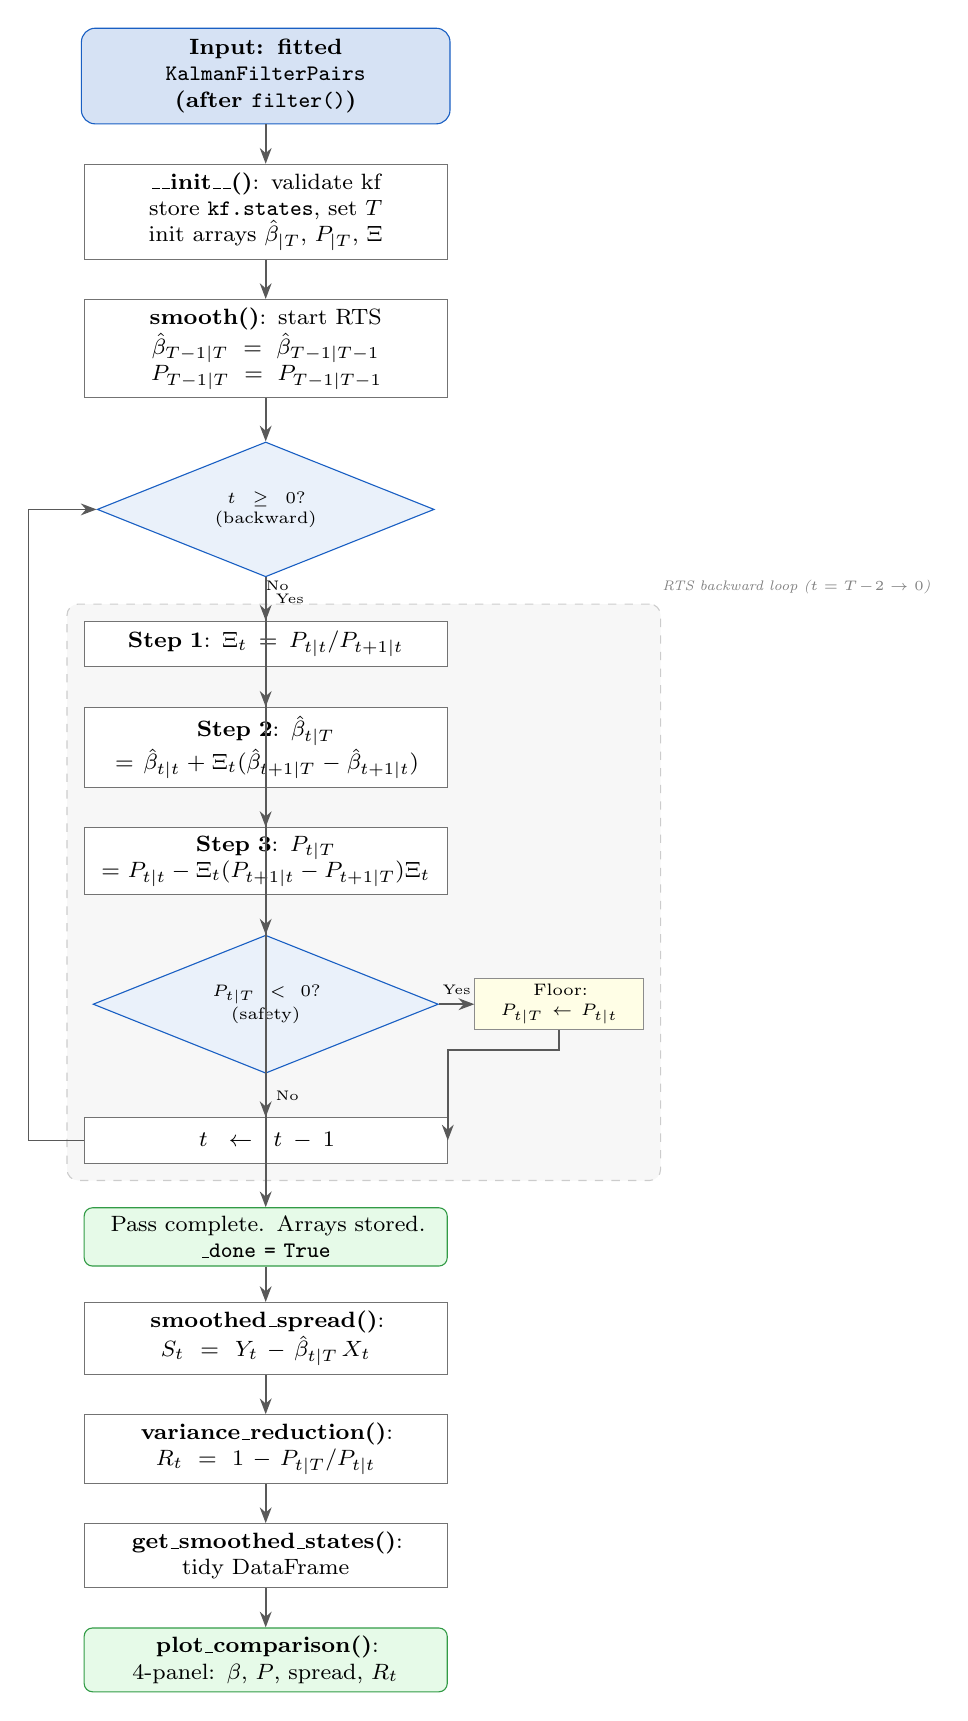
\begin{tikzpicture}[node distance=0.50cm,
                    every node/.style={font=\scriptsize}]

  \node (in) [fc_start]
    {Input: fitted \texttt{KalmanFilterPairs}\\(after \texttt{filter()})};

  \node (init) [fc_proc, below=of in]
    {\textbf{\_\_init\_\_()}: validate kf\\
     store \texttt{kf.states}, set $T$\\
     init arrays $\hat\beta_{|T}$, $P_{|T}$, $\Xi$};

  \node (smooth) [fc_proc, below=of init]
    {\textbf{smooth()}: start RTS\\
     $\hat\beta_{T-1|T}=\hat\beta_{T-1|T-1}$\\
     $P_{T-1|T}=P_{T-1|T-1}$};

  \node (loop) [fc_dec, below=0.55cm of smooth]
    {$t \geq 0$?\\(backward)};

  \node (gain) [fc_proc, below=0.55cm of loop]
    {\textbf{Step 1}: $\Xi_t = P_{t|t} / P_{t+1|t}$};

  \node (state) [fc_proc, below=of gain]
    {\textbf{Step 2}: $\hat\beta_{t|T}$\\
     $= \hat\beta_{t|t} + \Xi_t(\hat\beta_{t+1|T} - \hat\beta_{t+1|t})$};

  \node (cov) [fc_proc, below=of state]
    {\textbf{Step 3}: $P_{t|T}$\\
     $= P_{t|t} - \Xi_t(P_{t+1|t} - P_{t+1|T})\Xi_t$};

  \node (safe) [fc_dec, below=0.5cm of cov]
    {$P_{t|T} < 0$?\\(safety)};

  \node (floor) [fc_side, right=0.45cm of safe]
    {Floor:\\$P_{t|T}\leftarrow P_{t|t}$};

  \node (decr) [fc_proc, below=0.55cm of safe]
    {$t \leftarrow t - 1$};

  \node (done) [fc_out, below=0.55cm of decr]
    {Pass complete. Arrays stored.\\
     \texttt{\_done = True}};

  \node (spread) [fc_proc, below=0.45cm of done]
    {\textbf{smoothed\_spread()}:\\
     $S_t = Y_t - \hat\beta_{t|T}\,X_t$};

  \node (vr) [fc_proc, below=of spread]
    {\textbf{variance\_reduction()}:\\
     $R_t = 1 - P_{t|T}/P_{t|t}$};

  \node (df) [fc_proc, below=of vr]
    {\textbf{get\_smoothed\_states()}:\\
     tidy DataFrame};

  \node (plot) [fc_out, below=of df]
    {\textbf{plot\_comparison()}:\\
     4-panel: $\beta$, $P$, spread, $R_t$};

  \draw[arr] (in)   -- (init);
  \draw[arr] (init) -- (smooth);
  \draw[arr] (smooth)-- (loop);
  \draw[arr] (loop) -- node[right,font=\tiny]{Yes} (gain);
  \draw[arr] (gain) -- (state);
  \draw[arr] (state)-- (cov);
  \draw[arr] (cov)  -- (safe);
  \draw[arr] (safe) -- node[above,font=\tiny]{Yes} (floor);
  \draw[arr] (floor.south) -- ++(0,-0.25) -| (decr.east);
  \draw[arr] (safe) -- node[right,font=\tiny]{No} (decr);
  \draw[arr] (decr.west) -- ++(-0.7,0) |- (loop.west);
  \draw[arr] (loop.south) -- ++(0,-0.25)
    node[left,font=\tiny,xshift=12pt,yshift=4pt]{No}
    -- (done.north);
  \draw[arr] (done)  -- (spread);
  \draw[arr] (spread)-- (vr);
  \draw[arr] (vr)   -- (df);
  \draw[arr] (df)   -- (plot);

  \begin{pgfonlayer}{background}
    \node[draw=gray!40,fill=gray!6,dashed,rounded corners=4pt,
          fit=(gain)(state)(cov)(safe)(floor)(decr),
          inner sep=6pt,
          label={[font=\tiny\itshape,gray]above right:%
                 RTS backward loop ($t=T\!-\!2 \to 0$)}]
          (loopbox) {};
  \end{pgfonlayer}

\end{tikzpicture}%
}
\caption{Flowchart of \texttt{KalmanSmoother}.  Shaded region:
backward loop ($t=T-2$ down to $t=0$).  Left-side arrow is the
loop-back (decrement $t$).}
\label{fig:smoother_flow}
\end{figure}

%=============================================================================
\section{Python Implementation}
%=============================================================================

\subsection{Constructor: \texttt{\_\_init\_\_()}}

\begin{tcolorbox}[codebox={Constructor --- \texttt{\_\_init\_\_()}}]
\begin{lstlisting}[style=pythonplain]
class KalmanSmoother:
    """RTS Backward Smoother for dynamic beta."""
    def __init__(self, kf: KalmanFilterPairs):
        if not isinstance(kf, KalmanFilterPairs):
            raise TypeError("kf must be KalmanFilterPairs.")
        if not kf._fitted:
            raise RuntimeError("Must call filter() first.")
        self._kf             = kf
        self._states         = kf.states
        self.T               = len(self._states)
        self._smoothed_beta  = None
        self._smoothed_P     = None
        self._smoothing_gain = None
        self._done           = False
\end{lstlisting}
\end{tcolorbox}

\subsection{Core Backward Pass: \texttt{smooth()}}

\begin{tcolorbox}[codebox={Backward Pass --- \texttt{smooth()}}]
\begin{lstlisting}[style=pythonplain]
def smooth(self):
    T = self.T;  s = self._states
    sb = np.zeros(T);  sP = np.zeros(T)
    xi = np.zeros(T - 1)
    # Boundary: terminal smoothed = filtered
    sb[T-1] = s[T-1].beta
    sP[T-1] = s[T-1].P
    for t in range(T-2, -1, -1):   # backward
        P_t_t  = s[t].P            # P_{t|t}
        P_t1_t = s[t+1].P_pred     # P_{t+1|t}
        if P_t1_t <= 0:
            warnings.warn(f"P_t1_t<=0 at t={t}")
            gain = 0.0
        else:
            gain = P_t_t / P_t1_t   # Formula 1
        xi[t] = gain
        b_t1T = sb[t+1]             # beta_{t+1|T}
        b_t1t = s[t+1].beta_pred    # beta_{t+1|t}
        # Formula 2: smoothed state
        sb[t] = s[t].beta + gain * (b_t1T - b_t1t)
        P_t1T = sP[t+1]
        # Formula 3: smoothed covariance
        sP[t] = P_t_t - gain*(P_t1_t - P_t1T)*gain
        if sP[t] < 0:               # safety floor
            sP[t] = P_t_t
    self._smoothed_beta  = sb
    self._smoothed_P     = sP
    self._smoothing_gain = xi
    self._done = True
    return sb, sP
\end{lstlisting}
\end{tcolorbox}

\subsection{Derived Outputs}

\begin{tcolorbox}[codebox={Spread and Variance Reduction}]
\begin{lstlisting}[style=pythonplain]
def smoothed_spread(self) -> pd.Series:
    """S_t = Y_t - beta_{t|T} * X_t"""
    self._require_done("smoothed_spread")
    x = np.array([s.x for s in self._states])
    y = np.array([s.y for s in self._states])
    spread = y - self._smoothed_beta * x
    idx = (self._kf._y_index
           if hasattr(self._kf, "_y_index")
           else np.arange(self.T))
    return pd.Series(spread, index=idx,
                     name="smoothed_spread")

def variance_reduction(self) -> pd.Series:
    """R_t = 1 - P_{t|T} / P_{t|t}, clipped [0,1]"""
    self._require_done("variance_reduction")
    fP = np.array([s.P for s in self._states])
    R  = 1.0 - self._smoothed_P / np.maximum(fP, 1e-20)
    idx = (self._kf._y_index
           if hasattr(self._kf, "_y_index")
           else np.arange(self.T))
    return pd.Series(np.clip(R, 0, 1),
                     index=idx, name="variance_reduction")
\end{lstlisting}
\end{tcolorbox}

\subsection{Four-Panel Plot: \texttt{plot\_comparison()}}

\begin{tcolorbox}[codebox={Comparison Plot}]
\begin{lstlisting}[style=pythonplain]
def plot_comparison(self, figsize=(14,10)):
    """4-panel: beta, P, spread, variance reduction."""
    self._require_done("plot_comparison")
    df  = self.get_smoothed_states()
    vr  = self.variance_reduction()
    idx = df.index
    fig, axes = plt.subplots(4, 1, figsize=figsize,
                             sharex=True)
    # Panel 1: hedge ratio
    axes[0].plot(idx, df["filtered_beta"],
                 "steelblue", lw=0.9, alpha=0.7)
    axes[0].plot(idx, df["smoothed_beta"],
                 "crimson", lw=1.2)
    axes[0].fill_between(idx,
        df["smoothed_beta"]-2*np.sqrt(df["smoothed_P"]),
        df["smoothed_beta"]+2*np.sqrt(df["smoothed_P"]),
        alpha=0.12, color="crimson")
    # Panel 2: covariance
    axes[1].plot(idx, df["filtered_P"], "steelblue")
    axes[1].plot(idx, df["smoothed_P"], "crimson")
    # Panel 3: spread
    axes[2].plot(idx, df["filtered_spread"], "steelblue")
    axes[2].plot(idx, df["smoothed_spread"], "crimson")
    axes[2].axhline(0, color="k", lw=0.8, ls="--")
    # Panel 4: variance reduction (%)
    axes[3].fill_between(idx, 0, vr*100,
                          alpha=0.6, color="mediumseagreen")
    axes[3].set_ylabel("%")
    plt.tight_layout(); plt.show()
\end{lstlisting}
\end{tcolorbox}

%=============================================================================
\section{Connection to EM Parameter Estimation}
%=============================================================================

\subsection{Why the Smoother Feeds EM}

The EM algorithm for state-space models estimates
$\theta = (Q, R, \beta_0, P_0)$ via:

\begin{tcolorbox}[notebox={EM for State-Space (Shumway--Stoffer)}]
\textbf{E-step}: Given $\theta^{(k)}$, run KF \emph{and} RTS
smoother to compute:
\[
  \hat\beta_{t|T}^{(k)},\quad
  P_{t|T}^{(k)},\quad
  P_{t,t-1|T}^{(k)} \;\text{(cross-covariance)}
\]
\textbf{M-step}: Update $\theta^{(k+1)}$ to maximise the
expected complete-data log-likelihood
$\mathbb{E}_{\theta^{(k)}}[\log p(\beta_{0:T}, Y_{1:T} \mid \theta)]$.
\end{tcolorbox}

\noindent The smoother is essential in the E-step because the M-step
update for $Q$ involves $\mathbb{E}[(\beta_t-\beta_{t-1})^2 \mid Y_{1:T}]$,
which conditions on the \emph{full} dataset.

\subsection{EM Parameter Update Formulae}

\begin{tcolorbox}[mathbox={EM Updates from Smoothed States}]
\vspace{-4pt}
\begin{align}
  Q^{\text{new}} &= \frac{1}{T-1}\sum_{t=1}^{T-1}
    \Bigl[P_{t|T} + P_{t-1|T}
    - 2\Xi_{t-1}P_{t|T} \nonumber\\
  &\qquad\quad + (\hat\beta_{t|T}-\hat\beta_{t-1|T})^2\Bigr]
    \label{eq:Q_em}\\[4pt]
  R^{\text{new}} &= \frac{1}{T}\sum_{t=1}^{T}
    \bigl[(Y_t - \hat\beta_{t|T}X_t)^2
    + X_t^2\,P_{t|T}\bigr]
    \label{eq:R_em}
\end{align}
\vspace{-4pt}
These require smoothed (not filtered) quantities because they
condition on all $T$ observations.
\end{tcolorbox}

\subsection{Manual $Q$-Tuning via $\bar R$}

\begin{enumerate}\setlength\itemsep{1pt}
  \item Run filter with trial $Q_0$; run smoother.
  \item Compute $\bar{R} = T^{-1}\sum_t R_t$.
  \item $\bar{R} > 0.8$: $Q_0$ too small (over-confident filter).
        Increase $Q$.
  \item $\bar{R} < 0.05$: $Q_0$ too large (diffuse filter).
        Decrease $Q$.
  \item Target $\bar{R} \in [0.2, 0.6]$ for balanced smoothing.
\end{enumerate}

%=============================================================================
\section{Pipeline Position}
%=============================================================================

\subsection{Dark-Wing Step 6.1}

\begin{center}\small
\begin{tabular}{@{}clp{2.0cm}l@{}}
\toprule
\textbf{Step} & \textbf{Module} & \textbf{File / Class} & \textbf{Role}\\\midrule
1 & Data ingest    & \texttt{yfinance}            & Price download\\
2 & Log prices     & ---                          & $p_t = \ln P_t$\\
3 & Stationarity   & \texttt{ADF\_Test}           & Unit root\\
4 & Cointegration  & \texttt{JohansenTest}        & Pair select\\
5 & VECM           & \texttt{VECM}                & Error correct.\\
6 & Kalman Filter  & \texttt{KalmanFilterPairs}   & Forward pass\\
\textbf{6.1} & \textbf{RTS Smoother}
             & \textbf{\texttt{KalmanSmoother}}   & \textbf{Backward pass}\\
6.2 & Dyn.\ Beta   & \texttt{DynamicBeta}         & Beta analysis\\
7 & Signals        & \texttt{SignalGenerator}     & Entry/exit\\
8 & Backtest       & \texttt{BacktestEngine}      & PnL sim.\\
\bottomrule
\end{tabular}
\end{center}

\subsection{Input / Output Contract}

\begin{tcolorbox}[notebox={Interface Specification}]
\textbf{Input}: \texttt{KalmanFilterPairs} with
\texttt{\_fitted=True}.  Each \texttt{kf.states[t]} is a
\texttt{KalmanState} namedtuple with fields:
\texttt{beta}, \texttt{P}, \texttt{beta\_pred},
\texttt{P\_pred}, \texttt{x}, \texttt{y}.\\[4pt]
\textbf{Output} (after \texttt{smooth()}):
\begin{itemize}\setlength\itemsep{0pt}
  \item \texttt{\_smoothed\_beta} --- \texttt{ndarray} shape $(T,)$
  \item \texttt{\_smoothed\_P} --- \texttt{ndarray} shape $(T,)$
  \item \texttt{\_smoothing\_gain} --- \texttt{ndarray} shape $(T-1,)$
\end{itemize}
\textbf{Downstream}: \texttt{DynamicBeta} reads the
\texttt{get\_smoothed\_states()} DataFrame.
\end{tcolorbox}

\subsection{End-to-End Usage}

\begin{tcolorbox}[codebox={Pipeline Usage (RELIANCE / TCS)}]
\begin{lstlisting}[style=pythonplain]
import yfinance as yf, numpy as np
from kalman_filter import KalmanFilterPairs
from smoother import KalmanSmoother

# Download log prices
raw = yf.download(["RELIANCE.NS","TCS.NS"],
      start="2021-01-01",end="2024-01-01",
      auto_adjust=True)["Close"].dropna()
lp = np.log(raw)
y, x = lp["RELIANCE.NS"], lp["TCS.NS"]

# Forward pass: Kalman filter
kf = KalmanFilterPairs(Q=1e-5, R=1e-3)
kf.filter(y, x)

# Backward pass: RTS smoother (Step 6.1)
ks = KalmanSmoother(kf)
beta_s, P_s = ks.smooth()

# Summary statistics
ks.summary()

# Variance reduction
vr = ks.variance_reduction()
print(f"Mean R_t = {vr.mean()*100:.1f}%")

# Smoothed spread for backtest entry/exit
spread = ks.smoothed_spread()

# 4-panel diagnostic plot
ks.plot_comparison()
\end{lstlisting}
\end{tcolorbox}

%=============================================================================
\section{Mathematical Quick-Reference}
%=============================================================================

\begin{tcolorbox}[resultbox={All Formulae at a Glance}]
\textbf{State-Space Model}:
\[
  Y_t = \beta_t X_t + \varepsilon_t,\;\varepsilon_t\sim\mathcal{N}(0,R)
\]
\[
  \beta_t = \beta_{t-1} + \eta_t,\;\eta_t\sim\mathcal{N}(0,Q)
\]

\textbf{KF Prediction} (forward, $t=0\to T-1$):
\[
  \hat\beta_{t+1|t} = \hat\beta_{t|t},\quad
  P_{t+1|t} = P_{t|t} + Q
\]

\textbf{RTS Smoother} (backward, $t=T-2\to 0$):
\[
  \Xi_t = \frac{P_{t|t}}{P_{t+1|t}} \in (0,1]
\]
\[
  \hat\beta_{t|T} = \hat\beta_{t|t}
    + \Xi_t\,(\hat\beta_{t+1|T} - \hat\beta_{t+1|t})
\]
\[
  P_{t|T} = P_{t|t} - \Xi_t\,(P_{t+1|t} - P_{t+1|T})\,\Xi_t
\]

\textbf{Variance Reduction}: $R_t = 1 - P_{t|T}/P_{t|t} \in [0,1]$

\textbf{Smoothed Spread}: $S_t = Y_t - \hat\beta_{t|T}\,X_t$

\textbf{EM $Q$ update}: Eq.~\eqref{eq:Q_em} \quad
\textbf{EM $R$ update}: Eq.~\eqref{eq:R_em}
\end{tcolorbox}

%=============================================================================
\end{document}
